\subsection{Polarization Leakage from Feedhorn}

\paragraph{Description:}

Beam asymmetries from the feedhorn can cause leakage from temperature to polarization and E-modes to B-modes. The beams need to be modeled and measured so that they can be correctly incorporated into the analysis to minimize these effects.

\paragraph{Plan to model and/or measure:}
The simplest way to model this effect is by assuming a pair-differenced detector. Note that this is a simplified model that gives total polarization leakage, so not all the temperature to polarization leakage power goes into the B-modes. To better quantify this leakage, a full pipeline treatment of the beams with simulated maps and scan strategy is needed, but this calculation is a good check of the worst-case scenario that can be done internal to the TWGs. Based on symmetry arguments presented in Shimon et al., 2008~\cite{Shimon_2008}, the leakage from temperature into the B-modes has a large suppression factor compared to leakage into E-modes. Furthermore, accounting for beam asymmetries in analysis could further mitigate the leakage by an order of magnitude or more, cross-linking in the maps helps identify and quantify this leakage, and the use of a HWP would significantly mitigate the leakage.

The polarization leakages in the power spectra are estimated using the simulated co- and cross-polar beams from HFSS. Assuming a pair-differenced detector, the electric fields on the sky $E_x$ and $E_y$ are coupled to the electric field in the detectors $E_a$ and $E_b$ by
\begin{equation}\label{eqn:beams}
  \begin{bmatrix}
  E_a\\
  E_b
  \end{bmatrix}
  =
  \begin{bmatrix}
  \beta_{ax} & \beta_{ay}\\
  \beta_{bx} & \beta_{by}
  \end{bmatrix}
  \begin{bmatrix}
  E_x\\
  E_y
  \end{bmatrix}
  \,\,\, ,
\end{equation}
where $a$ and $x$ as well as $b$ and $y$ are aligned along the boresight. Here $\beta_{ax}$ and $\beta_{by}$ are the co-polar beams, and $\beta_{ay}$ and $\beta_{bx}$ are the cross-polar beams. The default setting in HFSS is to source the calculation through the wave port in the $x$ direction, which gives $\beta_{ax}$ and $\beta_{ay}$. To model $\beta_{bx}$ and $\beta_{by}$, the source must be changed to the wave port in the $y$ direction. The complex beams are then given by the sum of their real and imaginary parts as
\begin{align}
\beta_{nx} & =  \mathrm{Re}(rEL3X)+i\, \mathrm{Im}(rEL3X) \nonumber \\
\beta_{ny} & =  \mathrm{Re}(rEL3Y)+i\, \mathrm{Im}(rEL3Y)\,\,\,\,\,,
\end{align}
where $n$ is either $a$ or $b$. The co- and cross-polar beams from HFSS are then masked such that they go to zero outside of the Lyot stop, and a 2D FFT is performed to estimate the far field beams~\cite{Simon_Thesis_2016}.

For an ideal bolometer differencing pair at the output of the of the horn, the measured polarized signal $P$ would be
\begin{equation}\label{eqn:p1}
P=E_a-E_b \,\,\,\,.
\end{equation}
The Stokes parameters using the decreasing phase convention are given by
\begin{align}\label{eqn:Stokes}
I & =  |E_{x}|^2+ |E_{y}|^2  \nonumber \\
Q & =   |E_{x}|^2- |E_{y}|^2  \nonumber \\
U & =  2\,\mathrm{Re}(E_{x} E_{y}^{*}) \nonumber \\
V & =  2\,\mathrm{Im}(E_{x} E_{y}^{*})\,\,\,\,\,.
\end{align}
Here $I$ is the intensity, $Q$ and $U$ describe the linear polarization as defined in Equation~\ref{eqn:Stokes_QU}, and $V$ describes the circular polarization. Substituting Equation~\ref{eqn:beams} into Equation~\ref{eqn:p1} and using the definition of the Stokes parameters  as in Equation~\ref{eqn:Stokes} gives
\begin{equation}
P=\sigma I + \delta Q + \epsilon U+ \gamma V\,\,\,\, ,
\end{equation}
where the coefficients are the beam couplings from $I$, $Q$, $U$, and $V$ into $P$. For an ideal detector, $\delta=1$ and $\sigma=\epsilon=\gamma=0$. The beam couplings are then given by
\begin{align}\label{eqn:leakage beams}
\sigma & =  \frac{1}{2} (\beta_{ax}^2 + \beta_{ay}^2 - \beta_{bx}^2 - \beta_{by}^2) \\
\delta & =   \frac{1}{2} (\beta_{ax}^2 - \beta_{ay}^2 - \beta_{bx}^2 + \beta_{by}^2) \\
\epsilon & =  \mathrm{Re}(\beta_{ax}^{*} \beta_{ay} - \beta_{bx}\beta_{by}^{*} )  \\
\gamma & =  -\mathrm{Im}(\beta_{ax} \beta_{ay}^{*} + \beta_{bx}^{*}\beta_{by} )\,\,\,\,\,.
\end{align}
The beams are then normalized by the maximum of $\delta$ and averaged across the observation bands of each feedhorn. As the distance from the center of the array increases, the ellipticity of the Lyot stop as viewed from the pixel increases, which results in higher leakage. The central pixel thus gives the lowest temperature to polarization leakage. While edge pixels exhibit higher leakage, the average leakage beam of pairs of pixels equidistant from the array center on opposite sides of the array approximates the behavior of the central pixel. Therefore, the behavior of the central pixel can provide an estimate for the systematics of the array~\cite{Simon_Thesis_2016}.

To estimate the leakage in the power spectra from beam asymmetries, the window functions of the signal and leakage beams are calculated. For each beam, the magnitude squared of the FFT of the averaged far field beams is calculated and normalized by the maximum of the transformed $\delta$ beam. Next the 2D functions are binned radially to make a 1D window function.  To account for the rest of the telescope optics, one can normalize the multipole axis by comparing the $\delta$ window function to a window function of a Gaussian beam with full width at half maximum (FWHM) equal to that expected at a given center frequency of each observation band from optics modeling. The measured spectra are then determined by multiplying models of the EE and BB polarization spectra by the $\delta$ window function, the temperature to polarization leakage spectrum is determined by multiplying the modeled TT spectrum by the $\sigma$ window function, and the EE to BB leakage is determined by multiplying the modeled EE spectrum by the $\epsilon$ window function. An example of this for the AdvACT 150/230~GHz feedhorns is shown in Figures~\ref{fig:HF_measured_spectra}, \ref{fig:HF_TP_leakage}, and \ref{fig:HF_EB_leakage}~\cite{Simon_Thesis_2016}.

\begin{figure}[h!]
\centering
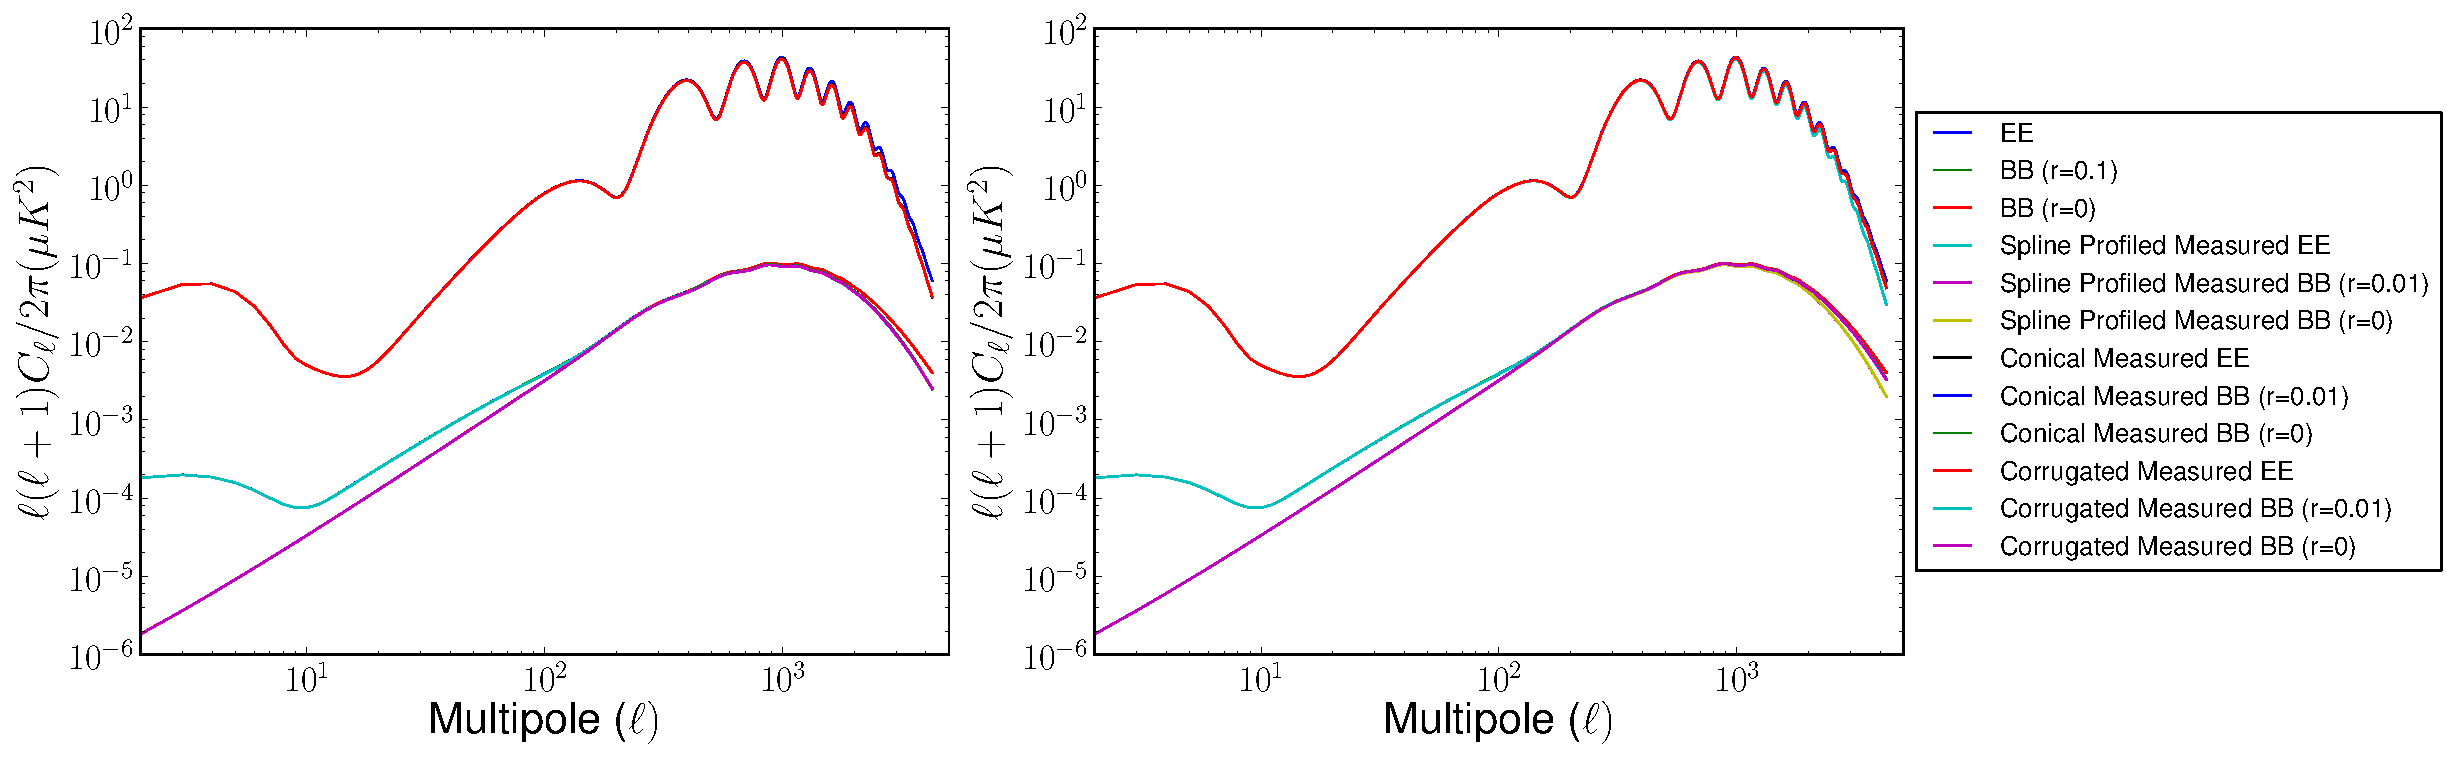
\includegraphics[width=\textwidth]{figures/HF_measured_spectra.pdf}
\caption{Simulated measurements of the EE and BB polarization spectra using the 150/230~GHz AdvACT feedhorn candidates are shown above for the 150~GHz band (left) and the 230~GHz band (right)~\cite{Simon_Thesis_2016}.}
\label{fig:HF_measured_spectra}
\end{figure}

\begin{figure}[h!]
\centering
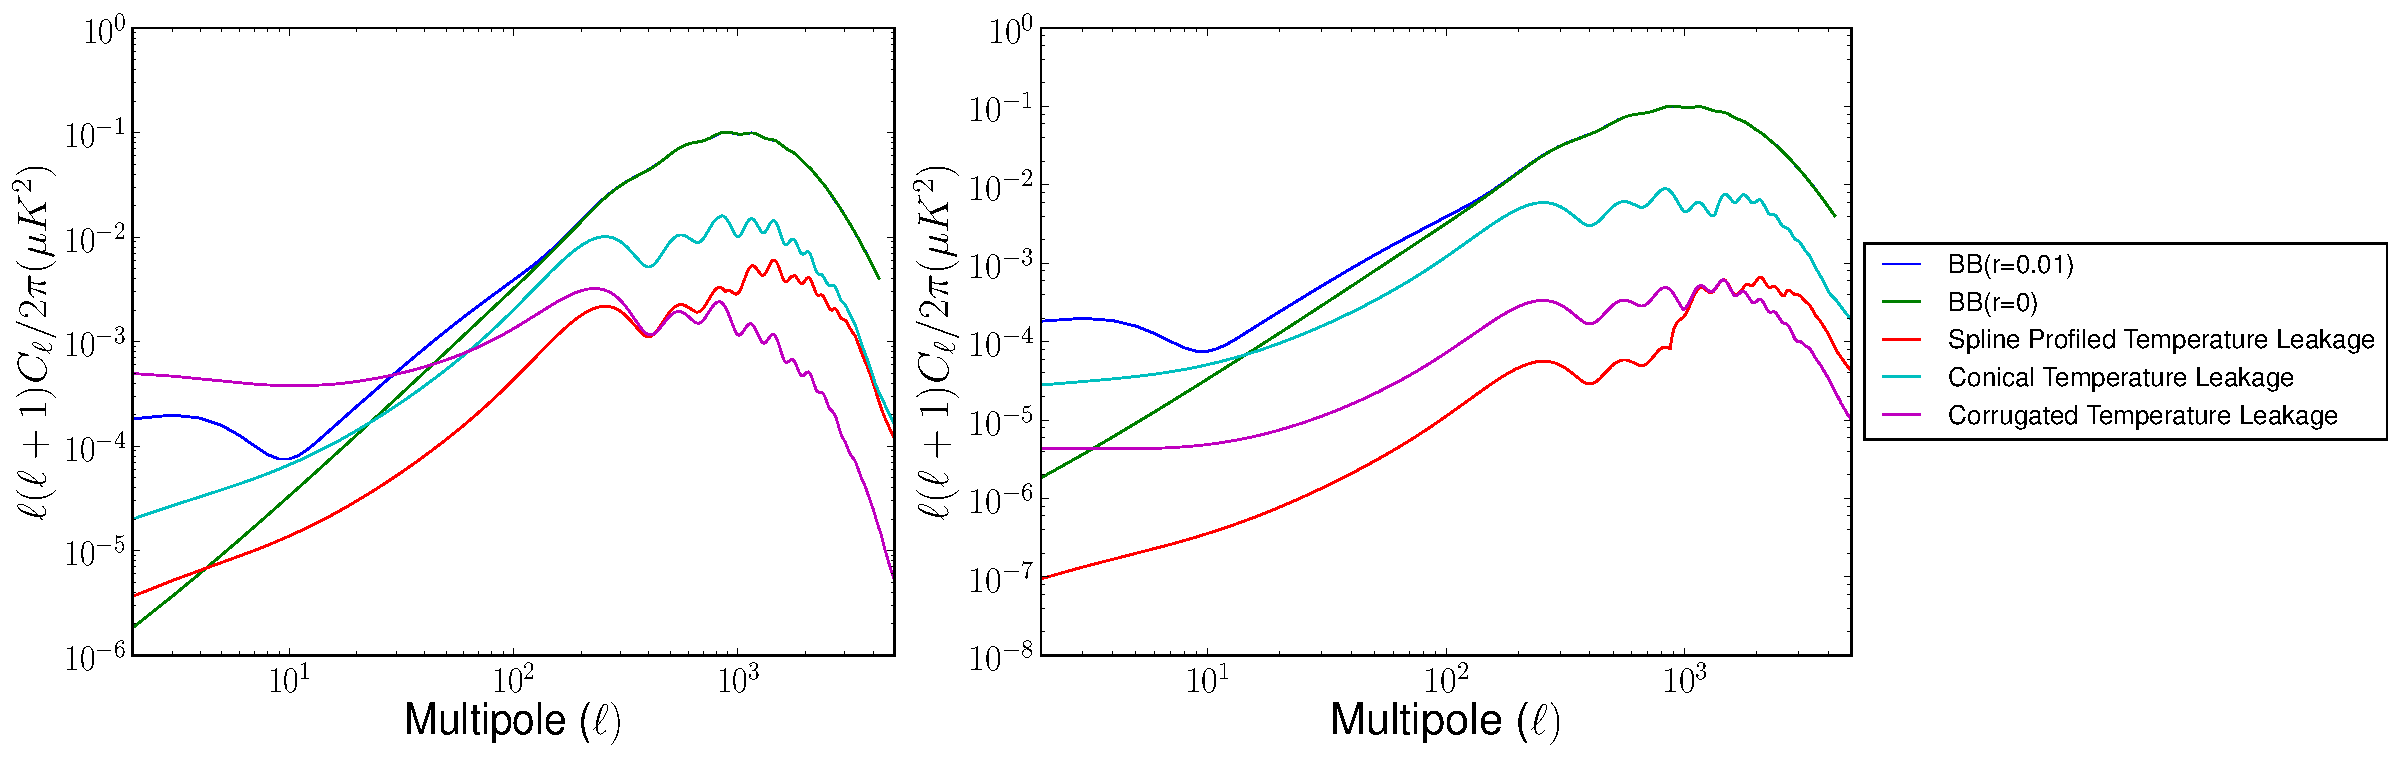
\includegraphics[width=\textwidth]{figures/HF_TP_leakage.pdf}
\caption{The temperature to polarization leakage of the AdvACT 150/230~GHz spline-profiled (red), conical (cyan), and corrugated (magenta) feedhorns are plotted with the B-mode signal for $r=0$ (green) and $r=0.01$ (blue) for the 150~GHz band (left) and the 230~GHz band (right)~\cite{Simon_Thesis_2016}.}
\label{fig:HF_TP_leakage}
\end{figure}

\begin{figure}[h!]
\centering
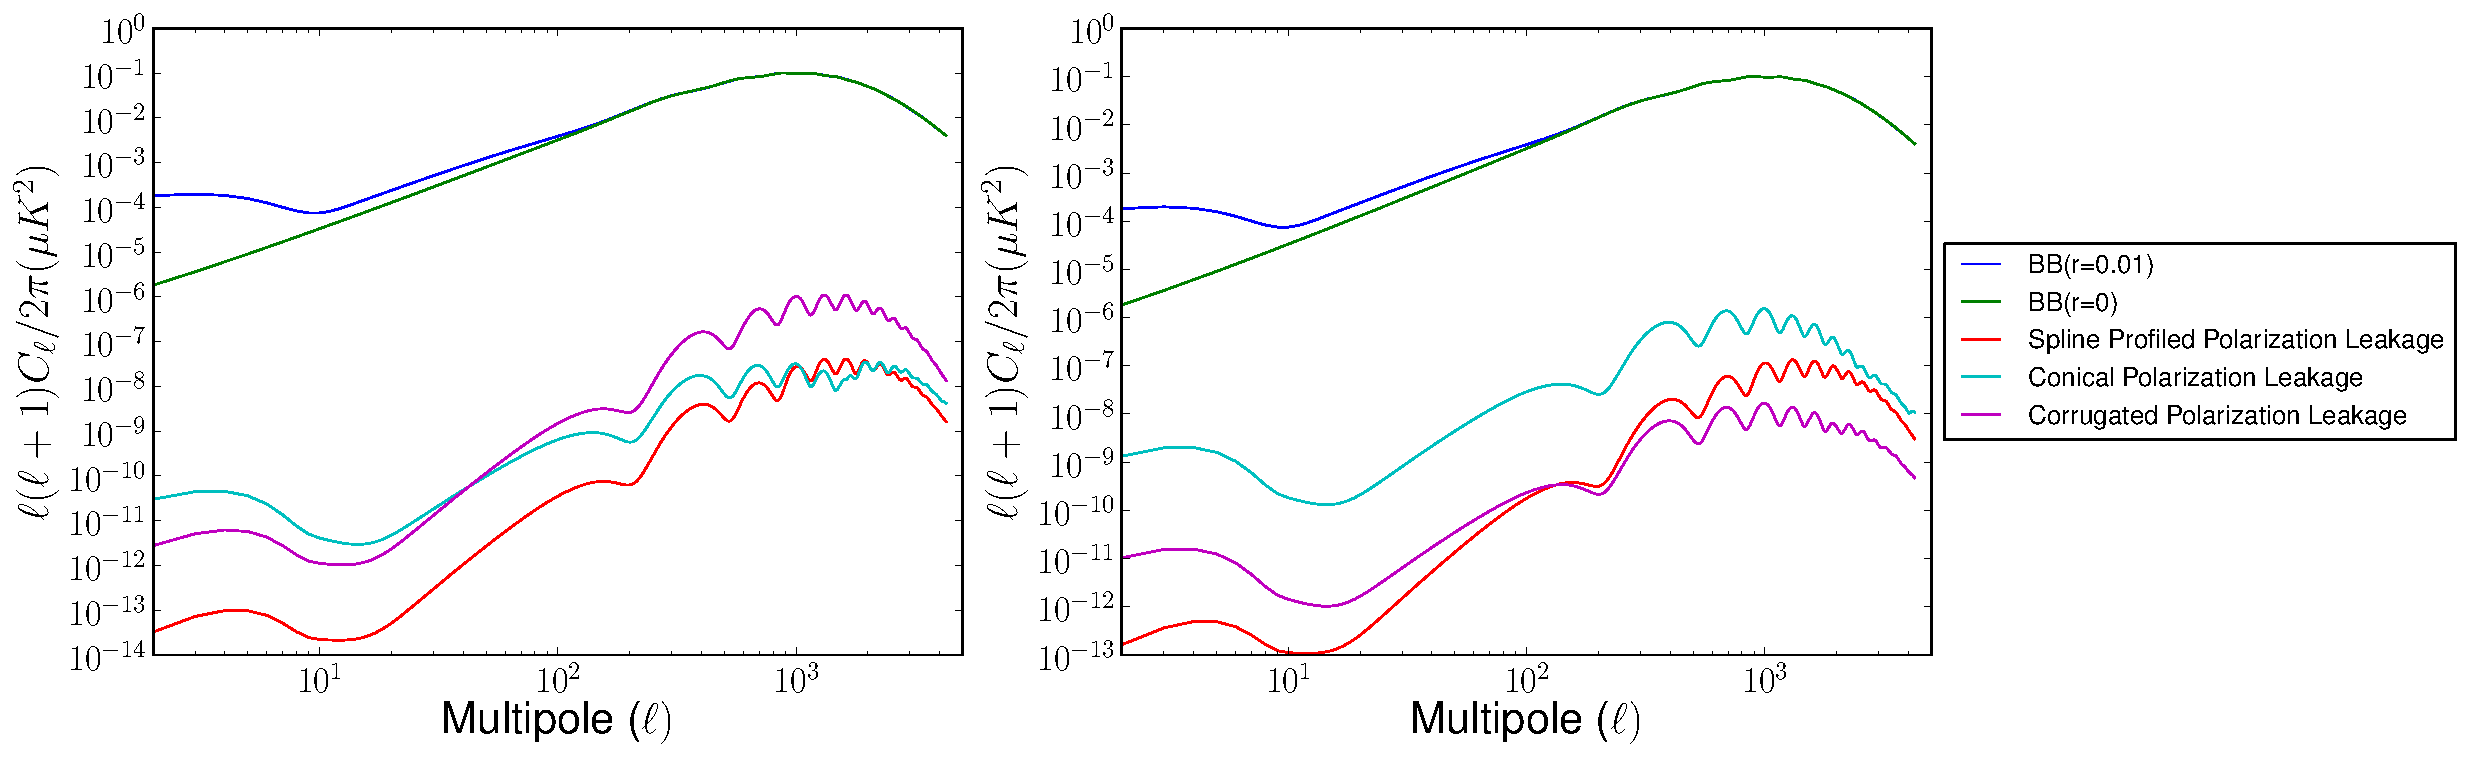
\includegraphics[width=\textwidth]{figures/HF_EB_leakage.pdf}
\caption{The EE to BB leakages of the AdvACT 150/230~GHz feedhorn candidates are shown above for the 150~GHz band (left) and the 230~GHz band (right). In all cases, this leakage is negligibly low~\cite{Simon_Thesis_2016}.}
\label{fig:HF_EB_leakage}
\end{figure}


\paragraph{Uncertainty/Range:}
This leakage must be lower than the B-mode signal by several orders of magnitude. The pair-differenced detector estimate above is an over-estimation by possibly an order of magnitude or more, so further modeling would need to be done from the SWG to get a more realistic value.

\paragraph{Parameterization:}
This can be parameterized with the estimated leakage spectra from the pair-differenced model or with the feedhorn beams from HFSS should more detailed modeling be desired.

